\documentclass{article}
\usepackage{overcite}
\usepackage{algorithm}
\usepackage{algorithmic}
\usepackage{subfigure}
\usepackage{listings} 
\usepackage{bm}
\usepackage{multirow}
\usepackage{url}
\usepackage{amsmath,amsfonts,amsthm,amssymb}
\usepackage{fancyhdr}
\usepackage{multirow}
\usepackage{extramarks}
\usepackage{chngpage}
\usepackage{color}
\usepackage{graphicx,float}
\usepackage{indentfirst}
\usepackage{bibentry,natbib}
\theoremstyle{plain} \newtheorem{theorem}{常识}[section]
\theoremstyle{plain} \newtheorem{lizi}{例}[section]
\newcommand{\Class}{Mathematics for Computer Science}

% Homework Specific Information. Change it to your own
\newcommand{\Title}{Homework 3}
\newcommand{\StudentName}{Huang Zhiao}
\newcommand{\StudentClass}{JK 40}
\newcommand{\StudentNumber}{2014011345}

% In case you need to adjust margins:
\topmargin=-0.45in      %
\evensidemargin=0in     %
\oddsidemargin=0in      %
\textwidth=6.5in        %
\textheight=9.0in       %
\headsep=0.25in         %

% Setup the header and footer
%\pagestyle{fancy}                                                       %
\lhead{\StudentName}                                                    %
\chead{\Title}                                                          %
\rhead{\firstxmark}                                                     %
\lfoot{\lastxmark}                                                      %
\cfoot{}                                                                %
\rfoot{Page\ \thepage\ of\ \protect\pageref{LastPage}}                  %
\renewcommand\headrulewidth{0.4pt}                                      %
\renewcommand\footrulewidth{0.4pt}                                      %

%%%%%%%%%%%%%%%%%%%%%%%%%%%%%%%%%%%%%%%%%%%%%%%%%%%%%%%%%%%%%
% Some tools
\newcommand{\enterProblemHeader}[1]{\nobreak\extramarks{#1}{#1 continued on next page\ldots}\nobreak%
                                    \nobreak\extramarks{#1 (continued)}{#1 continued on next page\ldots}\nobreak}%
\newcommand{\exitProblemHeader}[1]{\nobreak\extramarks{#1 (continued)}{#1 continued on next page\ldots}\nobreak%
                                   \nobreak\extramarks{#1}{}\nobreak}%

\newcommand{\homeworkProblemName}{}%
\newcounter{homeworkProblemCounter}%
\newenvironment{homeworkProblem}[1][Problem \arabic{homeworkProblemCounter}]%
  {\stepcounter{homeworkProblemCounter}%
   \renewcommand{\homeworkProblemName}{#1}%
   \section*{\homeworkProblemName}%
   \enterProblemHeader{\homeworkProblemName}}%
  {\exitProblemHeader{\homeworkProblemName}}%

\newcommand{\homeworkSectionName}{}%
\newlength{\homeworkSectionLabelLength}{}%
\newenvironment{homeworkSection}[1]%
  {% We put this space here to make sure we're not connected to the above.

   \renewcommand{\homeworkSectionName}{#1}%
   \settowidth{\homeworkSectionLabelLength}{\homeworkSectionName}%
   \addtolength{\homeworkSectionLabelLength}{0.25in}%
   \changetext{}{-\homeworkSectionLabelLength}{}{}{}%
   \subsection*{\homeworkSectionName}%
   \enterProblemHeader{\homeworkProblemName\ [\homeworkSectionName]}}%
  {\enterProblemHeader{\homeworkProblemName}%

   % We put the blank space above in order to make sure this margin
   % change doesn't happen too soon.
   \changetext{}{+\homeworkSectionLabelLength}{}{}{}}%

\newcommand{\Answer}{\ \\\textbf{Answer:} }
\newcommand{\Proof}{\ \\\textbf{Proof:} }
\newcommand{\Acknowledgements}[1]{\ \\{\bf Acknowledgements:} #1}
\newcommand{\Infer}{\Longrightarrow}
\newcommand{\ud}{\mathrm{d}}
\newcommand{\Reduce}{\Longleftarrow}
\newcommand{\Endproof}{\hfill $\Box$ \\}
\newcommand{\Real}{\mathbb{R}}
\newcommand*\circled[1]{\tikz[baseline=(char.base)]{\node[shape=circle,draw,inner sep=2pt] (char) {#1};}}

%%%%%%%%%%%%%%%%%%%%%%%%%%%%%%%%%%%%%%%%%%%%%%%%%%%%%%%%%%%%%


%%%%%%%%%%%%%%%%%%%%%%%%%%%%%%%%%%%%%%%%%%%%%%%%%%%%%%%%%%%%%
% Make title
\title{\textmd{\bf \Class: \Title}\\\normalsize\vspace{0.1in}}
%\date{} % --- if you de-comment \date{}, the date will not appear below the title
\author{\textbf{\StudentName}\ \ \StudentNumber}
%%%%%%%%%%%%%%%%%%%%%%%%%%%%%%%%%%%%%%%%%%%%%%%%%%%%%%%%%%%%%

\usepackage[colorlinks,linkcolor=red]{hyperref}


\usepackage[]{xeCJK}
%\setmainfont{Courier New} % 设置英文衬线字体
%\setCJKmainfont{} % 设置缺省中文字体


\begin{document}

\title{计算机组成与原理实验报告}
\author{计科40~~黄志翱~~2014011345}
\maketitle

\section{实验要求}
\subsection{一}
在Y86流水线处理器中增加IADDL(iaddl 立即数,目标寄存器)与LEAVE指令。

\subsection{二}
设计实现两个共享内存的Y86流水线处理器(各带私有的L1 Cache)间的数据通信。

\section{实验一}
\subsection{题意及解法分析}
\subsubsection{iaddl}
iaddl的作用为将一个常数加到一个指定的寄存器上,为了添加这个操作,我们需要做如下修改:

\begin{itemize}
    \item 在instr\_valid中将该操作添加为合法操作。
    \item 设置为需要寄存器和常数。
    \item 目标寄存器和B source设为D\_rB。
    \item ALU的两个操作数设为E\_valC和E\_valB。
    \item 设置为setcc。
\end{itemize}

\subsubsection{leave}
leave的等价代码为:

rrmovl \%ebp, \%esp

popl \%ebp

基本操作与pop类似,只不过是将\%esp寄存器的来源进行了修改,修改操作如下:

\begin{itemize}
    \item 在instr\_valid中将该操作添加为合法操作。
    \item 设置为需要寄存器。
    \item \%ebp作为A source和d\_dstM, \%esp作为B source和d\_dstM。
    \item ALU的两个操作数设为\%ebp和4。
    \item 将mem\_addr设为M\_valA。
    \item 在所有有popl的异常处理代码上添加上ileave。
\end{itemize}

\subsection{代码的测试}
对pipe-full.hcl进行修改后在ptest目录下进行make TFLAGS=-il进行测试,测试结果通过。

\section{实验二}
\subsection{题目分析}
显然该问题可以分为两个不同的问题。

\begin{itemize}
    \item 实现具有write-allocation-write-back的两个l1 cache,并实现两者通讯以达成缓存一致性。
    \item 基于共享内存实现Y86流水线之前的通讯。
\end{itemize}

我们只需要分别解决这两个问题即可。

\subsection{l1 cache}
首先详细地定义我们要实现的问题:在一个unix-like system下,我们需要实现两个进程。
每个进程,需要支持从内存中读取与向内存中写入。

缓存是一组键值对应的表,键指示内存中的位置,值则对应于存储在内存上的一个块(为了表述的简单,下面不妨设键由内存地址唯一指定,值就是一位)。

由于需要维护cache,所以向内存读取的方式被限定为:查找被访问的地址是否在缓存中,若在,则读取,否则从内存将相应的内容加载到缓存,读取。

由于要求write-allocation-write-back,所以向内存写入的方式被限定为:查找被访问的地址是否在缓存中,若在,则直接在缓存中写入,否则从内存将相应的内容加载到缓存,写入。另外,当缓存满时,需要将某个缓存中的元素写入内存以进行替换。

对于多进程的情况下,我们需要加入如下两个约束:

\begin{itemize}
    \item 对于内存中同一位置的写入不能同时进行。
    \item 从缓存中读取时所得到的值必须是正确的。
\end{itemize}

在此前提下尽可能少减少向内存的写入和读取操作。为了实现这个目的,我采取了经典的MESI协议。

\subsubsection{MESI}
在MESI中,我们要求如果有某个元素存在于两个缓存上,则这两个缓存上的内容必须一致。

具体而言,对于一个缓存的一个键值,存在四种状态:

\begin{itemize}
    \item M,该位置有效,键被该进程独占,值与内存中不同。
    \item E,该位置有效,键被该进程独占,值与内存中相同。
    \item S,两个进程都存有此值,且两个缓存,内存中的值都是一致的。
    \item I,此位置的缓存无效。
\end{itemize}

假定两个进程之间能够通讯,现在进程A想做一点事情,那么我们可以很容易地凭借这些状态对内存进行操作:

\begin{itemize}
    \item 若当前位置是M,则A可以直接操作而当做B不存在。
    \item 若当前位置是E,则A可以直接操作而当做B不存在。
    \item 若当前位置是S,如果A是读操作,可以直接读取而当B不存在,如果A要写,则A需要通知B放弃该值,将状态改为I。
    \item 若当前位置是I,A需要通知B,若该值在B以M状态存在,则B需要将值写入内存,A将其加载进入缓存。如果A是读取,则A,B状态都是S,如果A是写入,则A状态变为M,B状态变为I。
\end{itemize}

\subsubsection{cache通讯}
A, B之间通讯依赖于bus的存在。基本方法是:A和B随时监听对方的信号,当A想要对B进行任何信息交流时,A发出信号。一旦B空闲下来了,就回答A的请求。此时A即可将所要发出的任意数量的信息提供给B,A每次等待B接收信息处理。这样通讯直到最后A发出结束信号,双方结束通讯。

具体实现上,bus是一块共享内存,A和B分别了bus的不同部位。A发出的任何信号在bus上表现是将特定的位数置0或者置1。A,B通过轮询的方式等待对方的通讯:

如果A和B同时发出请求,则让编号大的回答标号较小的防止死锁。

还有一个值得注意的细节是,由于rmmovl和mrmovl的设计,我们对内存的访问很多时候都是连续四个进行的,为了使得能够保证在读取的时候四个内存的值都不会修改,我采取了将对方一直锁住,然后进行连续四次操作的方法。

理论上而言,由于一个block的大小通常都会超过4,故而实际上只要双方能够对至多两个cache line进行同步即可---但考虑到block为1的时候这个方法会退化到需要同步四个cache line,于是我并未这么实现。

通讯的相关代码是misc/cache/cache.h的ask和answer函数。

\subsubsection{block的处理}
假设cache line的block大小为64,那么我们可以通过对地址右移六位求得对应的block,之后所有cache到内存与从内存到cache的所有操作都对block同时操作即可。

理论上在cache中寻找指定的元素应该通过散列表进行,但考虑到实际上cache的大小通常非常小,为了写代码方便我使用for循环进行了替代。

\subsubsection{实现细节}
cache相关的代码位于misc/cache/中。

cache.h中存放了缓存的实现与相关接口。

server.c提供两个cache共享的内存mem和总线bus。内存通过shmat相关函数获得。内存id由ftok函数指定,id信息被存放在shareinfo.h以供所有文件访问。

cache.c则实现了一个cache。首先根据shareinfo.h申请访问mem和bus。然后利用id得知自己是A还是B(从硬件角度上来讲,两个cache本身一定是有区分的,所以这个id在程序启动时就指定了),开一个共享内存$msg_{id}$,监听$msg_{id}$中是否有读写请求。当收到一个请求后,就利用MESI协议进行操作。监听msg和监听bus交替进行。无论何时收到请求则立刻回答。

在运行时,server, cache0, cache1,将会依次启动。之后只需要利用msg数组即可实现任何程序和cpu的交互接口:

\begin{lstlisting}[language=C]
//length表示我希望在一次操作中对连续多少个内存位进行处理。
//msg为通讯所使用的共享内存。
//answer表示回答另个一个缓存的询问。
//ONE_STEP为一次ask操作。

//server:
...
    while(1){
        answer(c);
        if(msg[0]){
            if(msg[0]==1){
                //Read
                int pos = msg[1];
                int ans = ONE_STEP(c, pos, 0, READ, msg[4]);
                msg[3] = ans;
                msg[0] = 0;
            }
...


//client
int read_request(volatile int* msg, int pos, int length){
    msg[1] = pos;
    msg[0] = 1;
    msg[4] = length;
    while(msg[0]){
    }
    return msg[3];
}

\end{lstlisting}

\subsection{对psim的修改}
\subsubsection{同时运行两个处理器}
假定两个cache进程已经运行,则cpu往内存进行的读写操作都通过msg发出请求进行即可。从这个角度看,只要cpu通过编号确定与哪个cache连接即可,剩下的操作与单核cpu完全一致。

所以第一步修改就是将isa.c中所有涉及到内存读写的get\_word\_val, get\_byte\_val, set\_word\_val, set\_byte\_val, load\_mem中所有对content的读写替换成通过msg向cache发出读写请求。

为了实现这些操作,我在cache\_rec类中添加了一个msg指针,指向共享内存(如果该指针为NULL则表示该对象是表示寄存器。)利用之前提供的交互,一段典型的get\_word\_val代码则可以写成:

\begin{lstlisting}[language=C]
bool_t get_word_val(mem_t m, word_t pos, word_t *dest)
{
    int i;
    word_t val;
    if(m->msg!=NULL){
        *dest = read_request(m->msg, pos, 4);
        return 1;
    }
    val = 0;
    for (i = 0; i < 4; i++)
        val = val | m->contents[pos+i]<<(8*i);
    *dest = val;
    return TRUE;
}
\end{lstlisting}

值得注意的是,此时如果用两个模拟器同时运行程序的话,load\_mem会将两个代码加载在同一个地方,所以我还修改了相应的函数和读取代码阶段valp的值将代码放置在不同的内存地址。但是由于本题只会运行两份相同的代码,所以这么做没有任何意义。

基于对这些操作的修改,实际上我们已经完成了两个cpu的并行。

\subsubsection{原子操作test}
为了使得运行相同代码时代码能够得知自己的身份,我加入了原子操作test:
$$test\ addr,reg$$
效果为读取addr的值,将值赋给reg,同时将addr处的值加1。

改代码格式与mrmovl基本类似,所以在修改pip-full.hcl时只要在所有有mrmovl的地方添加上该操作即可,但是区别在于test还有一个叫做mem\_test的信号量。

为了使得这个操作在是原子的,我们需要让cache也支持这个操作——这是非常容易的,我们可以将对内存地址的test看成read和write的组合,也就是进行连续8此的缓存操作即可。

为了在psim中使得该操作是连续的,需要同时修改mem阶段和wb阶段,因为这里面同时涉及到了对内存的读写与对寄存器的赋值。

对于mem阶段,需要加入如下代码:
\begin{lstlisting}[language=C]
...
    if (read && !mem_test) {
...
    if (mem_test && read){
        mem_test_address = mem_addr;
        int ans = test_memory(mem, mem_test_address);
        valm = ans;
    }
...
\end{lstlisting}

然后在写回阶段:
\begin{lstlisting}[language=C]
...
    if(wb_testM != REG_NONE){
        set_reg_val(reg, wb_testM, wb_valM);
        //为了视觉效果,我在test中加入了往屏幕输出test结果的功能。
        printf("PSIM_ID %d test_result:  %d on %d\n", PSIM_ID, wb_valM, mem_test_address);
    }
...
\end{lstlisting}
其中wb\_testM的值与wb\_destM一样,而mem\_test\_address是用于调试的全局变量,。

\subsection{y86 code}
当psim写好后,基本上y86代码就非常简单了。

代码流程如下:根据对指定内存的test决定是A还是B,跳到指定的代码段。

A会进行多次循环,每次循环是往连续的内存段中写入1,1的个数从1024到1024-100。写完之后会通过一个内存byte通知B已经写完。等待B回信,对特定的内存位test,输出test结果,继续循环。

B会等待A发出询问,当A询问完毕,会从特定内存位置开始遍历,数1的个数,累积求和,直到读取到内存中的值为0结束。

y86测试代码为pipe/ans.ys。

\subsection{代码的运行已经运行结果}
在总目录下进行make即可。

cd pipe, 进入pipe文件夹。在终端键入python3 run\_two\_sim.py即可运行。run\_two\_sim.py是一段python脚本,负责调用多个线程(server, cache 0, cache 1, psim 0, psim 1)。

程序会依次从1024输出到925,运行的视觉效果如图:

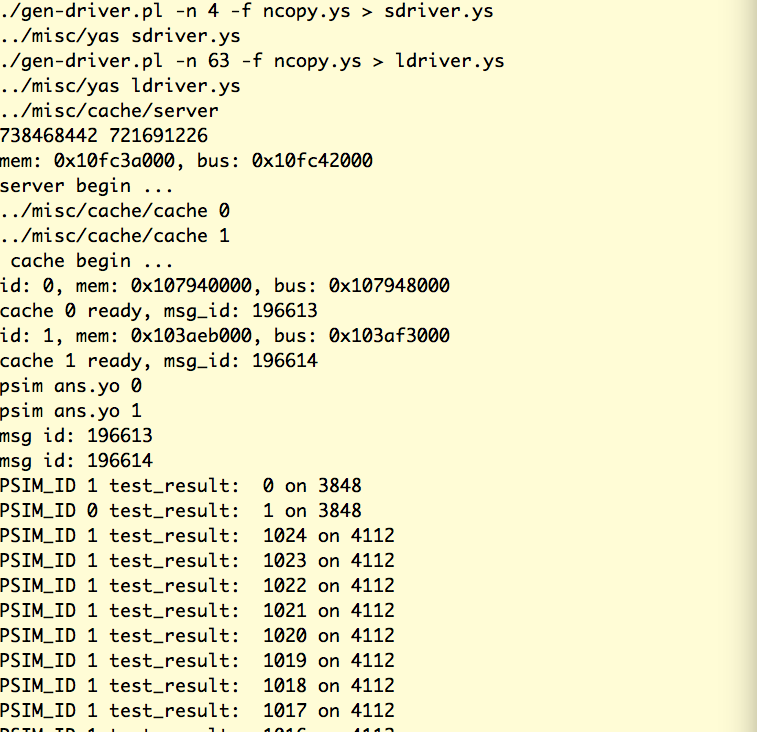
\includegraphics[scale=0.3]{1.png}
\section{感谢}
感谢茅佳源同学,在做第二个实验时和他进行的讨论给了我莫大的帮助。

也感谢这门课布置了这么一个好玩的实验。
\end{document}
